\section{Results}
\label{sec:results}

We wrote a simple CLI program to evaluate the algorithm under different conditions.
The program allows to set the input dimensions, the number of errors to introduce
and whether they should be collinear or not,
the simulated maximum amount of global memory, and the buffering strategy to use.
Several minor debugging parameters can be set, but they are out of the scope of this paper.

We tested the four strategies on a Quadro K620 desktop GPU. An important thing to consider is that display GPUs have a timeout on kernel executions, so we couldn't run tests with very large matrices. In any case, we believe that for bigger matrices the calculated performance should increase asymptotically.

When it came to profiling, the Nsight Compute suite was only available for the newer Ampere architecture, and for this GPU (Maxwell architecture), nvprof didn't have support for performance counters. For this reason we embedded some sort of profiling in the program itself.

As performance metrics, we used the overall execution time of the program (both total CPU and CUDA only), the total floating point arithmetic intensity and the average program performance (calculated as the total floating point operations over the total CUDA time).

To calculate the total floating point operations and the associated transfers to and from global memory (to then calculate the arithmetic intensity), we manually calculated the floating point operations number and associated global memory transfers count for each kernel we wrote. The program registers each kernel call and adds its float operations and transfers count to their respective counter.

To calculate the effective compute time we use CUDA events to register the start and end of the program (getting the total CUDA time with respect to the default stream).
To calculate the average performance we divide the total float operations by the total CUDA time, as a higher value indicate a higher use of the compute queue.
To calculate the total intensity we divide the total float operations by the total transfer count.

With that said, we hereby present our considerations on the obtained results.
We launched the same multiplication for the four different strategies, with inputs $20000 \times 2000$ and $2000 \times 2000$ (around 320MB of required memory), with the available global memory constrained to 10MB.

\begin{figure}[h]
	\centering
	\minipage{.481\textwidth}
	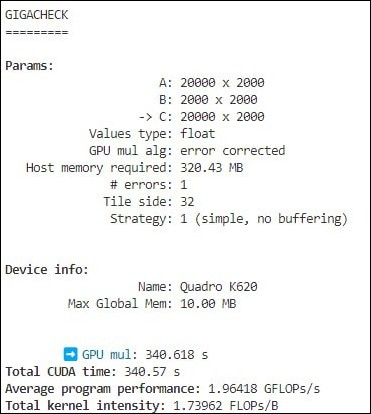
\includegraphics[width=\textwidth]{images/result_s1}
	\caption*{Strategy 1}
	\endminipage\hfill
	\minipage{.49\textwidth}
	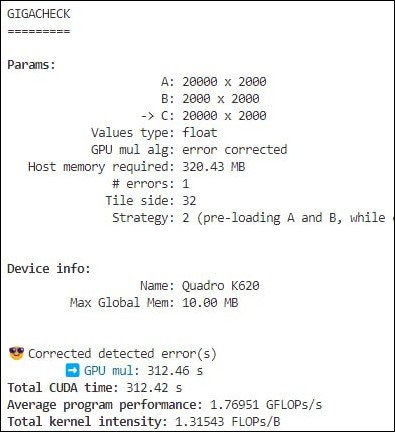
\includegraphics[width=\textwidth]{images/result_s2}
	\caption*{Strategy 2}
	\endminipage\hfill
	\linebreak
	\vspace{.02\textwidth}
	\linebreak
	\minipage{.481\textwidth}
	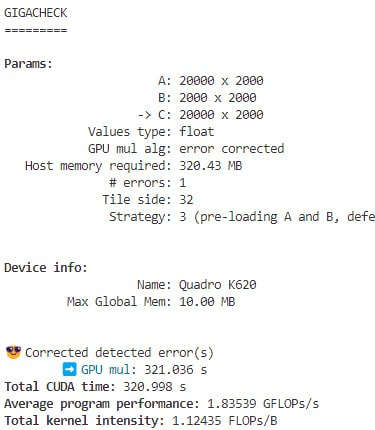
\includegraphics[width=\textwidth]{images/result_s3}
	\caption*{Strategy 3}
	\endminipage\hfill
	\minipage{.49\textwidth}
	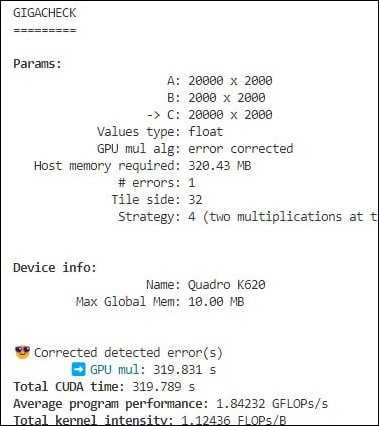
\includegraphics[width=\textwidth]{images/result_s4}
	\caption*{Strategy 4}
	\endminipage\hfill
	\caption{\centering results for the different strategies}\label{img:results-strategies}
\end{figure}

We see that, in comparison to strategy 1, strategy 2 has a slightly worse performance and intensity, but takes less overall time, as conjectured in \ref{img:strategies-timing-diagram}.

Strategy 3 has a similar performance to strategy 1 while taking less time, but a similar low intensity to strategy 2, to which it takes more time in comparison.

Strategy 4 is very similar to strategy 3 as expected, revealing that our concurrent kernel hypotesis was true.

TODO: considerazioni


\begin{figure}[h]
	\centering
	\minipage{.49\textwidth}
	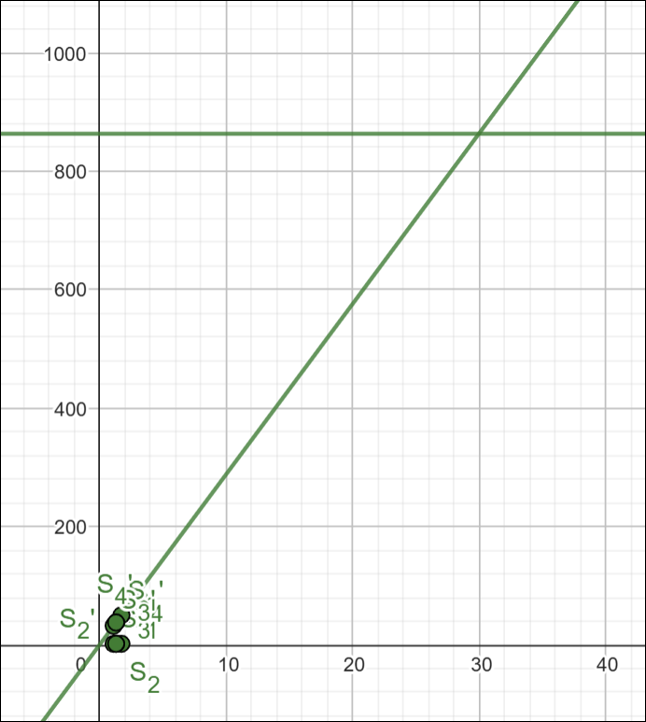
\includegraphics[width=\textwidth]{images/roofline-overview}
	\caption*{(a)}
	\endminipage\hfill
	\minipage{.49\textwidth}
	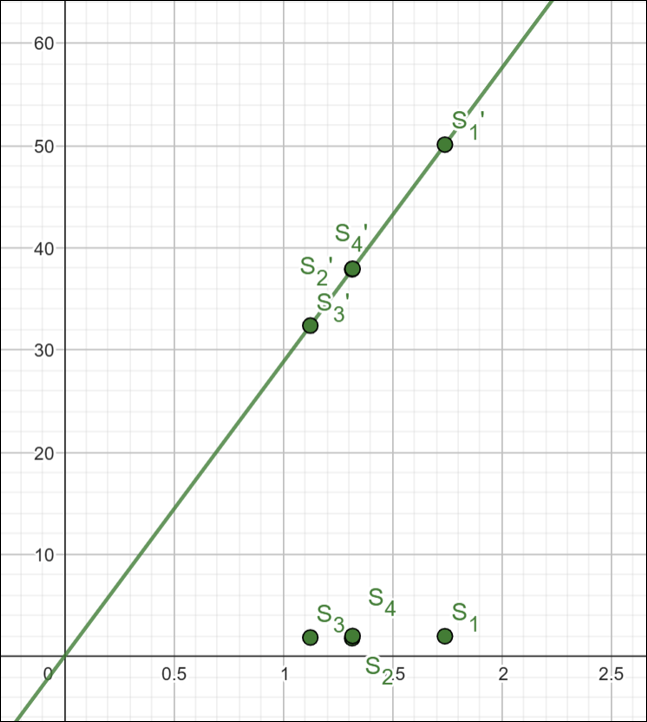
\includegraphics[width=\textwidth]{images/roofline-zoom.png}
	\caption*{(b)}
	\endminipage\hfill
	\caption{\centering Roofline model, (a) complete and (b) zoomed on the area where our program stands}\label{img:roofline-model}
\end{figure}
